\documentclass[]{beamer}
\usepackage[T1]{fontenc}
\usepackage[utf8]{inputenc}
\usepackage{lmodern}
\usepackage[italian]{babel}

\title{Il computer}
\author{\texorpdfstring{Mattia Cozzi\newline\href{mailto:cozzimattia@gmail.com}{\texttt{cozzimattia@gmail.com}}}{Mattia Cozzi}}
\date{a.s.~2023/2024}


%\documentclass[handout]{beamer}     %usare questa classe per generare l'handout

%\usepackage{pdfpages}   %per mostrare più quadri nella stessa pagina
%\pgfpagesuselayout{4 on 1}[a4paper,border shrink=5mm,landscape]


\usetheme{Singapore}
%\useoutertheme[left]{sidebar} %elementi intorno alle diapositive
\setbeamercovered{dynamic} %modifica l'aspetto del testo grigetto delle diapositive future. Argomenti: invisible/transparent/dynamic

%COLORE PRINCIPALE
\definecolor{verde}{RGB}{2, 194, 117} % UBC Blue (primary)
\setbeamercolor{structure}{fg=verde} % itemize, enumerate, etc
\setbeamercolor{alerted text}{fg=verde}


\usecolortheme{orchid}

\usepackage{tikz}
\usetikzlibrary{shapes.geometric, arrows}


\tikzstyle{startstop} = [ellipse, rounded corners, minimum width=3cm, minimum height=1cm,text centered, draw=black, fill=viola!30,text=white]
\tikzstyle{io} = [trapezium, trapezium left angle=70, trapezium right angle=110, minimum width=3cm, minimum height=1cm, text centered, draw=black, fill=viola!30,text=white]
\tikzstyle{process} = [rectangle, minimum width=3cm, minimum height=1cm, text centered, draw=black, fill=viola!30,text=white]
\tikzstyle{decision} = [diamond, minimum width=3cm, minimum height=1cm, aspect=2, text centered, draw=black, fill=viola!30,text=white]
\tikzstyle{arrow} = [thick,->,>=stealth]


\begin{document}

\begin{frame}
  \titlepage
\end{frame}


\begin{frame}
\frametitle{Contenuti}
\tableofcontents
\end{frame}

\section{Introduzione}

\begin{frame}
\frametitle{Definizioni}
\begin{block}{Computer}
  Il computer è una macchina elettronica capace di ricevere, trasmettere, memorizzare e soprattutto elaborare informazioni sotto forma di \emph{dati}.
\end{block}\pause

~

\begin{block}{Hardware}
  L'hardware è l'insieme delle parti elettroniche e meccaniche che compongono fisicamente il computer
\end{block}\pause

~

\begin{block}{Software}
  Il software è l'insieme delle parti immateriali a livello logico di un calcolatore (ad esempio un programma).
\end{block}
\end{frame}



\begin{frame}
\frametitle{Hardware (1)}
I componenti dell'hardware sono generalmente racchiusi dentro ad un \emph{case}{\pause} e sono, ad esempio:
\begin{columns}
  \begin{column}{0.4\textwidth}
    \begin{itemize}
      \item scheda madre;\pause
      \item CPU;\pause
      \item alimentatore elettrico;\pause
      \item memoria primaria (RAM);\pause
    \end{itemize}
    \end{column}
  \begin{column}{0.4\textwidth}
    \begin{itemize}
      \item memoria di massa;\pause
      \item scheda di rete;\pause
      \item scheda video;\pause
      \item scheda audio.
    \end{itemize}
    \end{column}
\end{columns}
\end{frame}



\begin{frame}
\frametitle{Hardware (2)}
\begin{figure}
  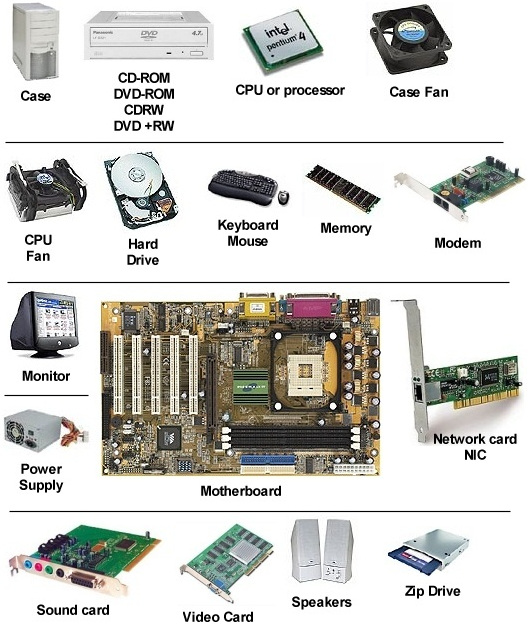
\includegraphics[width=.5\columnwidth]{img/hardware2.jpg}
\end{figure}
\end{frame}





\begin{frame}
\frametitle{Dati}
Un calcolatore riceve una serie di dati (sequenze di numeri e lettere) in ingresso, \alert<1>{esegue delle operazioni} su di essi e restituisce altri dati in uscita.\pause

~

I dati in ingresso sono chiamati in generale \alert<2>{input}.\pause

~

I dati in uscita sono chiamati invece \alert<3>{output}.
\end{frame}


\section{Von Neumann}


\begin{frame}
\frametitle{Architettura di Von Neumann (1)}
Lo schema generale secondo cui è costruito un calcolatore è detto \alert<1>{schema logico-funzionale di Von Neumann}.\pause

~

I componenti di questa architettura sono:
\begin{itemize}
  \item una \alert<2->{unità centrale di elaborazione} (CPU, \emph{central processing unit}), suddivisa in:\pause
  \begin{itemize}
    \item una \alert<3>{unità aritmetica logica} (ALU), cioè il componente che esegue i calcoli;\pause
    \item una \alert<4>{unità di controllo}, che coordina il calcolo;\pause
  \end{itemize}
  \item una \alert<5->{memoria centrale o primaria} (RAM, \emph{Random Access Memory}), che contiene i dati che stanno venendo utilizzati;\pause
  \item una o più \alert<6>{unità di I/O} (input/output), per fornire e leggere i dati (rientrano in questa categoria le memorie di massa o memorie secondarie).
\end{itemize}
\end{frame}



\begin{frame}
\frametitle{Architettura di Von Neumann (2)}
\begin{figure}
  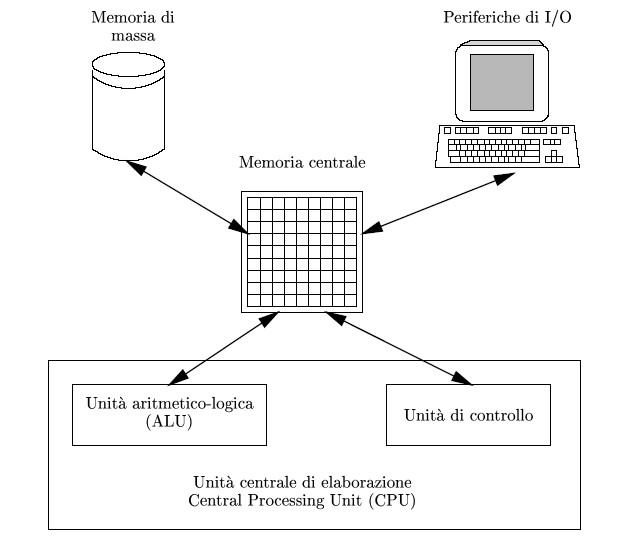
\includegraphics[width=.7\columnwidth]{img/vonneumann.jpg}
\end{figure}
\end{frame}




\section{Processore}


\begin{frame}
\frametitle{CPU}
\begin{figure}
  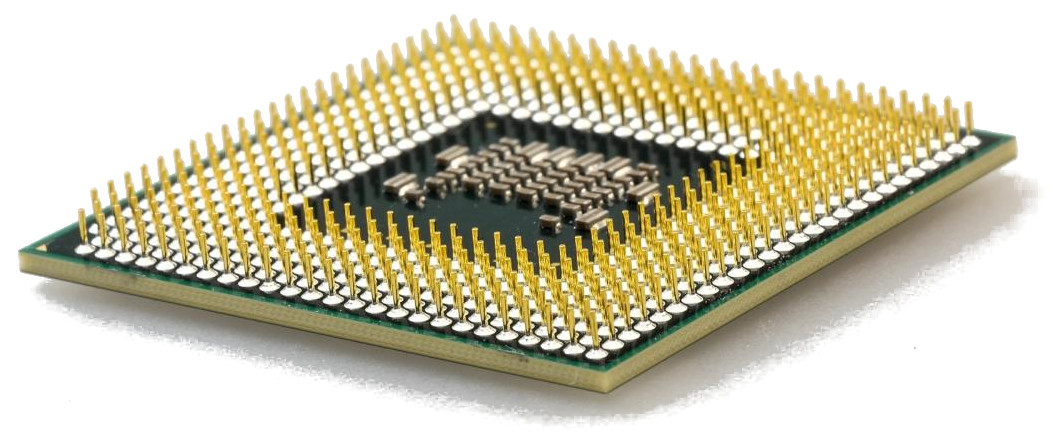
\includegraphics[width=.4\columnwidth]{img/cpu.jpg}
\end{figure}
La CPU, detta comunemente \alert<1>{processore}, è il componente del computer che esegue le operazioni aritmetiche e logiche che permettono il funzionamento della macchina.\pause

~

La CPU esegue il codice presente nella ROM (\emph{Read Only Memory}) in fase di avvio del sistema.\pause

~

Quando deve eseguire un programma, lo preleva dalla memoria di massa/secondaria (l'hard disk) e lo sposta nella RAM.
\end{frame}


\begin{frame}
\frametitle{Velocità del processore}
La velocità di un processore nell'eseguire operazioni è detta \alert<1>{velocità o frequenza di clock}. Viene solitamente misurata in \emph{hertz (Hz)}.\pause

~

Il computer Z1, costruito nel 1938, aveva una frequenza di clock massima di $ 1 \, Hz $, cioè eseguiva un'operazione (cioè una commutazione tra lo stato 0 e lo stato 1) al secondo.\pause

~

Le CPU attuali raggiungono una frequenza di clock di $ 4 \, GHz $, ovvero riescono ad eseguire fino a \alert<3>{4 miliardi di commutazioni al secondo}.\pause

~

Esistono anche \alert<4>{unità di elaborazione secondarie}, come schede audio, schede video, schede di rete, ecc.
\end{frame}

\section{Memorie}

\begin{frame}
\frametitle{Memoria centrale (RAM)}
\begin{figure}
  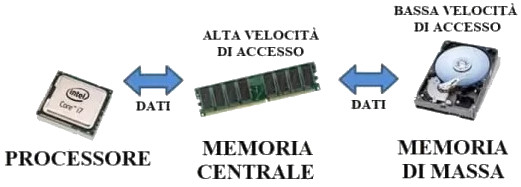
\includegraphics[width=.5\columnwidth]{img/memorie.jpg}
\end{figure}
La memoria centrale o primaria (RAM) è un tipo di \alert<1>{memoria ad alta velocità di accesso} che contiene i dati di cui la CPU ha bisogno per eseguire le operazioni.\pause

~

\alert<2>{Maggiore è la RAM, maggiore è la quantità di dati che in un certo istante il computer può gestire.} Se un computer ha poca RAM, non potremo aprire molte applicazioni contemporaneamente.\pause

~

Un computer casalingo ha tra i 4 e gli 8 GB di RAM.
\end{frame}


\begin{frame}
\frametitle{\emph{Read Only Memory} (ROM)}
\begin{figure}
  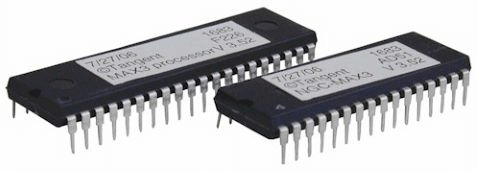
\includegraphics[width=.5\columnwidth]{img/rom.png}
\end{figure}
I dati presenti in RAM vengono scritti e sovrascritti molto rapidamente (la RAM è una \alert<1>{memoria volatile}).\pause

~

Quando i dati non devono mai essere modificati o ciò accade molto raramente, vengono immagazzinati in una \alert<2>{memoria di sola lettura}.\pause

~

Vengono immagazzinati in ROM i dati necessari all'avvio della macchina e quelli relativi al \alert<3>{sistema operativo}.
\end{frame}


\begin{frame}
\frametitle{Hard disk drive (HDD)}
\begin{figure}
  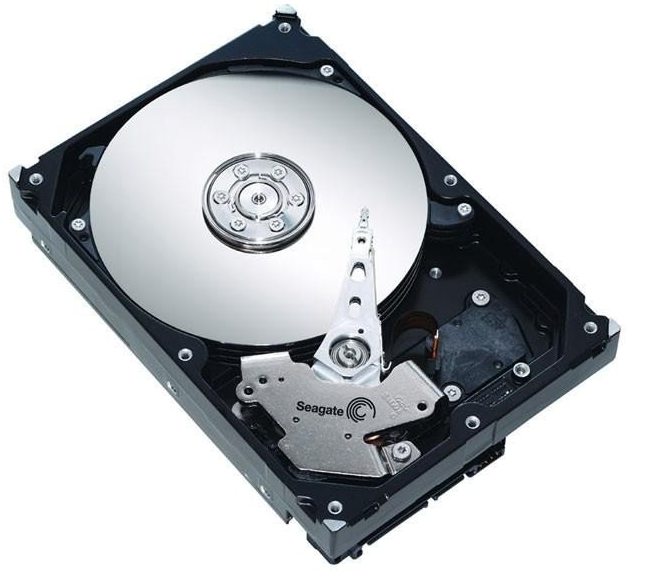
\includegraphics[width=.3\columnwidth]{img/hdd.png}
\end{figure}
Il disco rigido è il principale \alert<1>{dispositivo di archiviazione} a lungo termine di un computer.\pause

~

Vengono immagazzinati qui i programmi e i vari altri dati (musica, video, fotografie, ecc.). Gli HDD moderni possono contenere anche diversi terabyte di dati. \pause

~

Sono più lenti della RAM, ma i dati su essi possono essere facilmente cancellati e riscritti. La velocità varia in base al tipo di disco rigido.
\end{frame}


\begin{frame}
\frametitle{Dispositivi di archiviazione}
\begin{columns}
\begin{column}{.3\textwidth}
  \begin{center}
    Hard disk classico
    \begin{figure}
      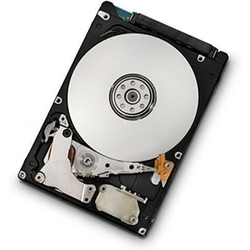
\includegraphics[width=\columnwidth]{img/hdd.jpg}
    \end{figure}
  \end{center}
\end{column}
\begin{column}{.3\textwidth}
  \begin{center}
    SSD
    \begin{figure}
      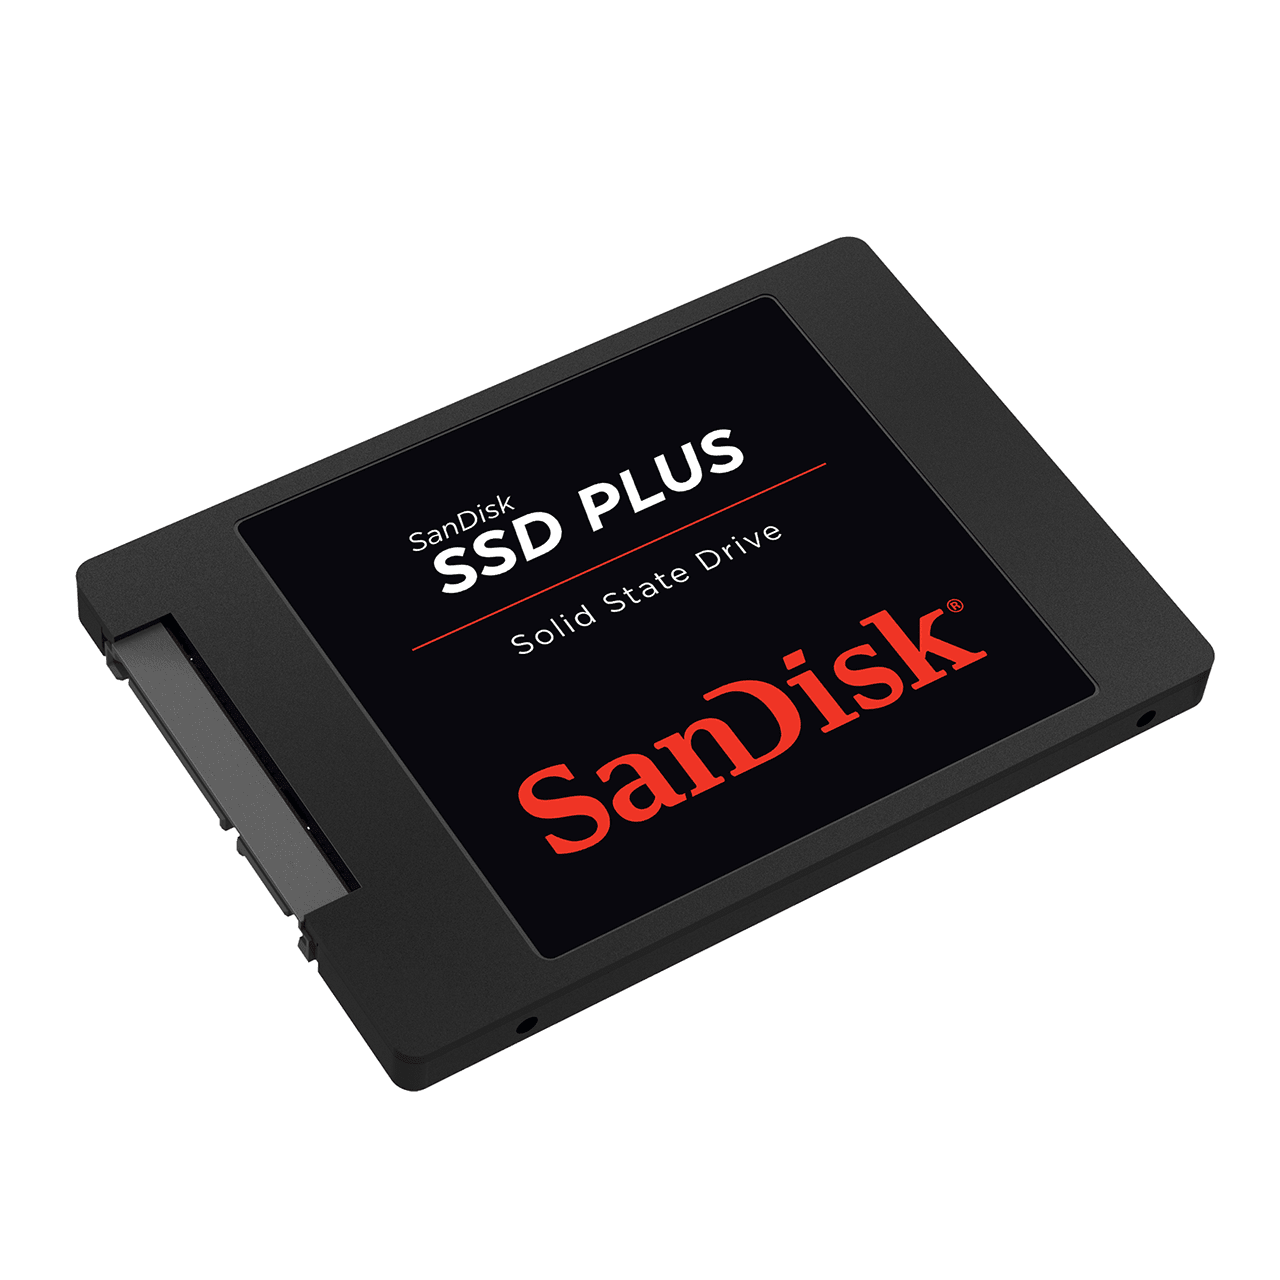
\includegraphics[width=\columnwidth]{img/ssd.png}
    \end{figure}
  \end{center}
\end{column}
\begin{column}{.3\textwidth}
  \begin{center}
    MicroSD
    \begin{figure}
      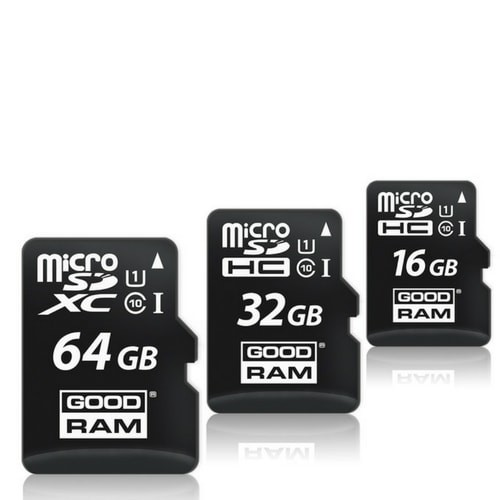
\includegraphics[width=\columnwidth]{img/microsd.jpg}
    \end{figure}
  \end{center}
\end{column}
\end{columns}
\end{frame}



\begin{frame}
\frametitle{Il \emph{file system}}
Il \emph{file system} è la \alert<1>{struttura con cui i dati sono organizzati su una memoria di massa}. Sono tipicamente settori affiancati del disco da 512 byte l'uno.\pause

~

\begin{columns}
  \begin{column}{.65\textwidth}
    Esso permette la memorizzazione, l'\alert<2>{organizzazione gerarchica}, l'accesso e la manipolazione dei dati che vi sono contenuti (esattamente come un buon archivio cartaceo).\pause
    
    ~
    
    Il file system viene rappresentato graficamente e manipolato con un \alert<3>{file browser}.
  \end{column}
  \begin{column}{.3\textwidth}
      \begin{figure}
        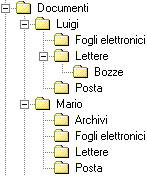
\includegraphics[width=\columnwidth]{img/albero.png}
      \end{figure}
  \end{column}
\end{columns}
\end{frame}




\begin{frame}
\frametitle{Metafore}
\begin{columns}
\begin{column}{.3\textwidth}
  \begin{center}
  CPU
  \begin{figure}
    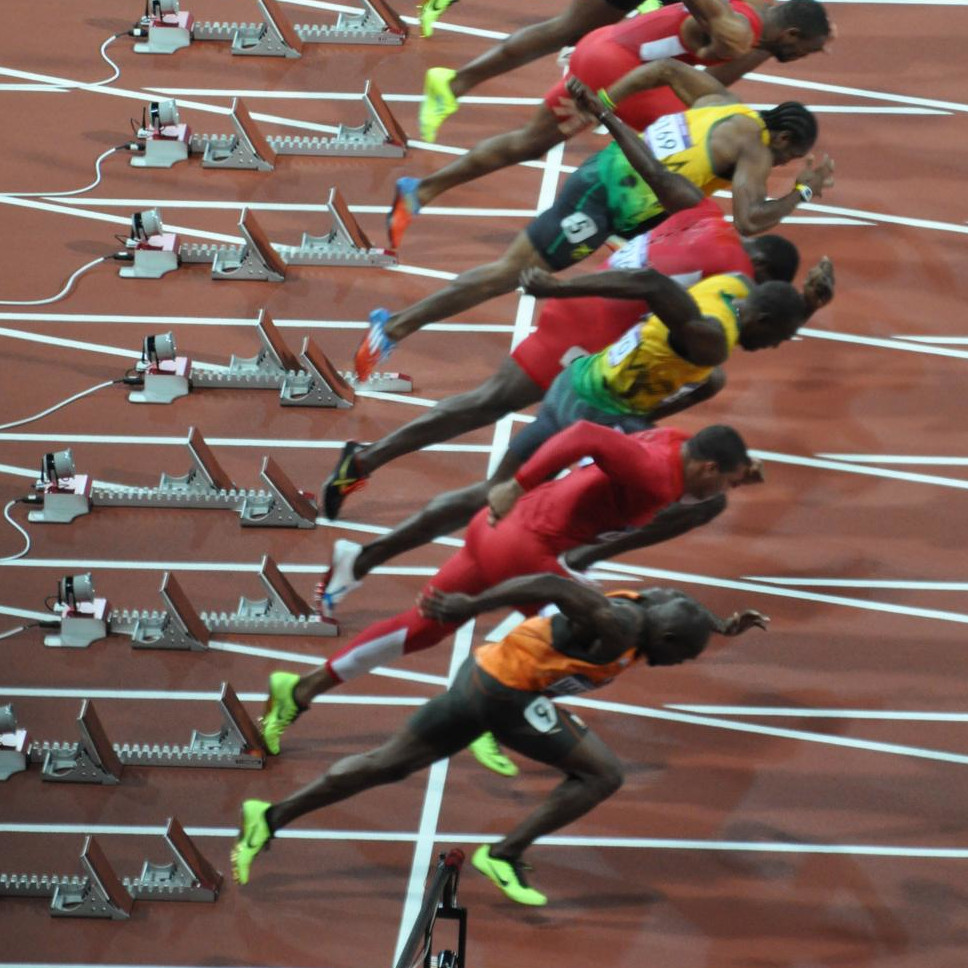
\includegraphics[width=\columnwidth]{img/sprint.jpg}
  \end{figure}
  La sua velocità si misura in GHz
  \end{center}
\end{column}
\begin{column}{.3\textwidth}
  \begin{center}
    RAM
    \begin{figure}
      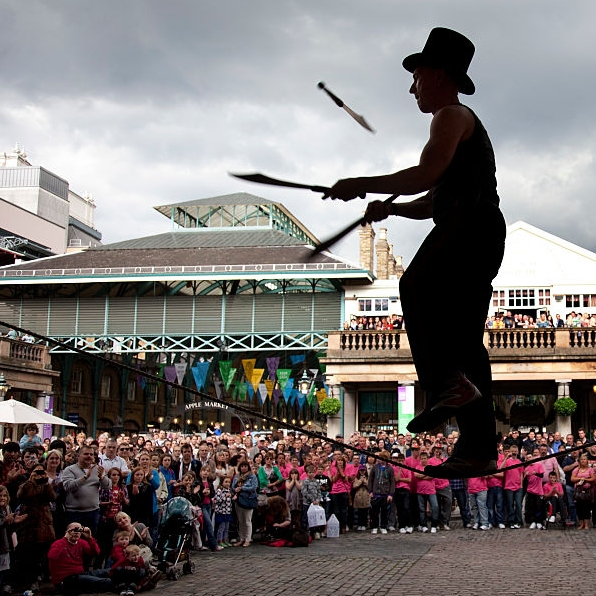
\includegraphics[width=\columnwidth]{img/giocoliere.jpg}
    \end{figure}
    La sua capacità si misura in GB
    \end{center}
\end{column}
\begin{column}{.3\textwidth}
  \begin{center}
    HDD 
    \begin{figure}
      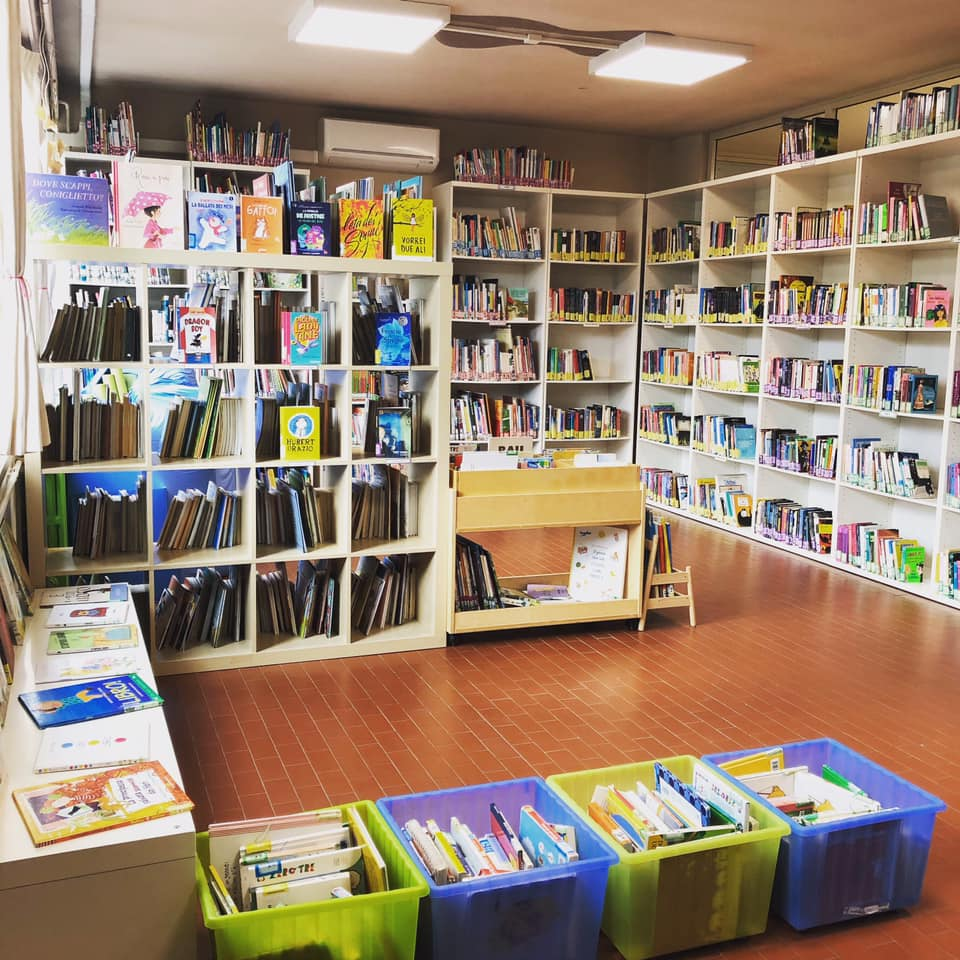
\includegraphics[width=\columnwidth]{img/biblioteca.jpg}
    \end{figure}
    La sua capacità si misura in GB o TB
    \end{center}
\end{column}
\end{columns}
\end{frame}

\section{I/O}


\begin{frame}
\frametitle{Periferiche di input}
In generale una \alert<1>{periferica} è un dispositivo hardware che viene collegato alla scheda madre, su cui è alloggiata la CPU.

~

Alcune periferiche servono per \alert<1>{fornire dati alla macchina} e sono dette periferiche di input.

~

\begin{columns}
\begin{column}{.22\textwidth}
  \begin{center}
  \begin{figure}
    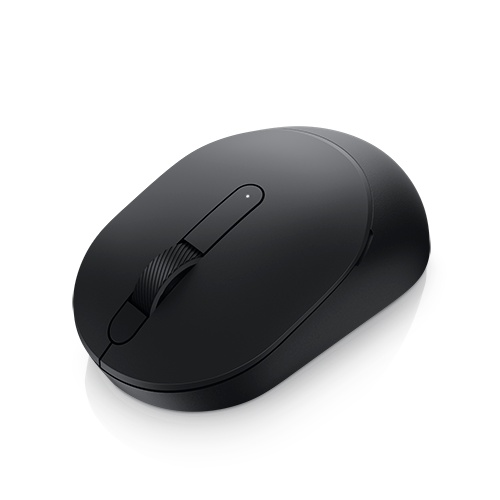
\includegraphics[width=\columnwidth]{img/mouse.jpg}
  \end{figure}
  Mouse
  \end{center}
\end{column}
\begin{column}{.22\textwidth}
  \begin{center}
    \begin{figure}
      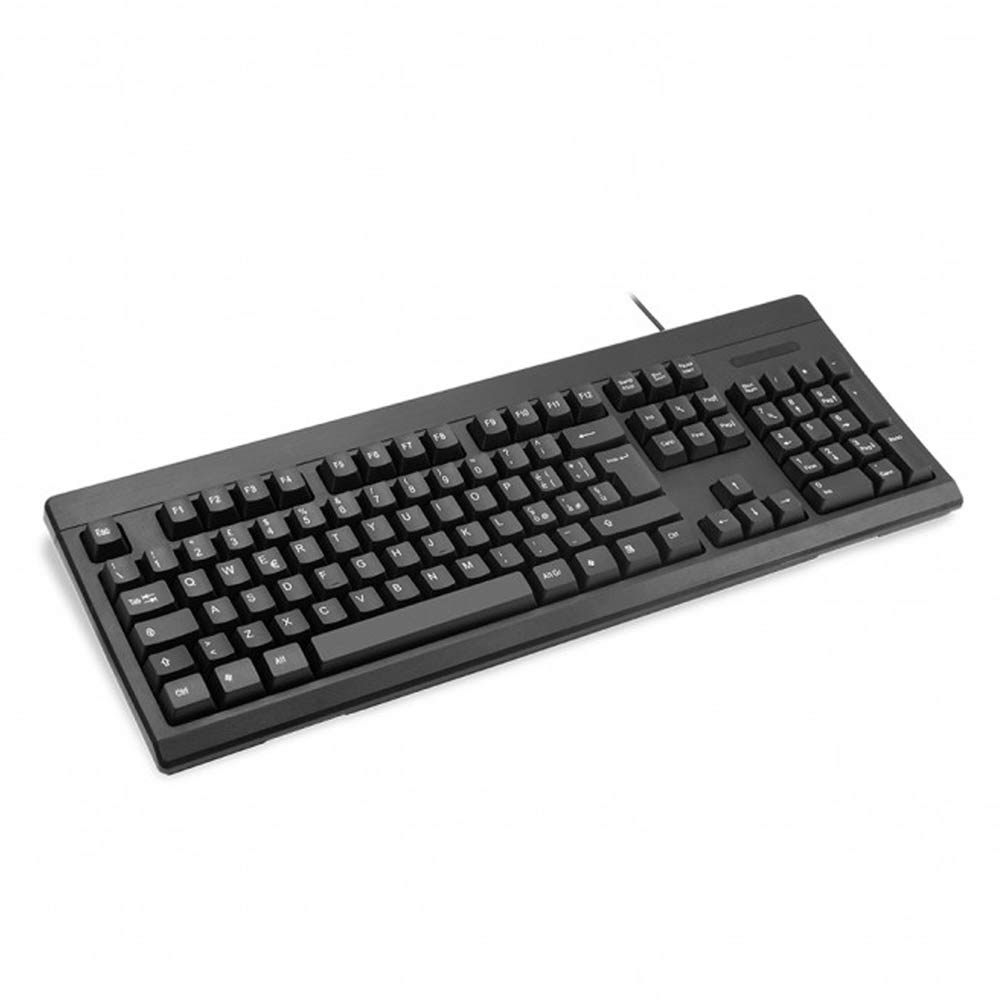
\includegraphics[width=\columnwidth]{img/tastiera.jpg}
    \end{figure}
    Tastiera
    \end{center}
\end{column}
\begin{column}{.22\textwidth}
  \begin{center} 
    \begin{figure}
      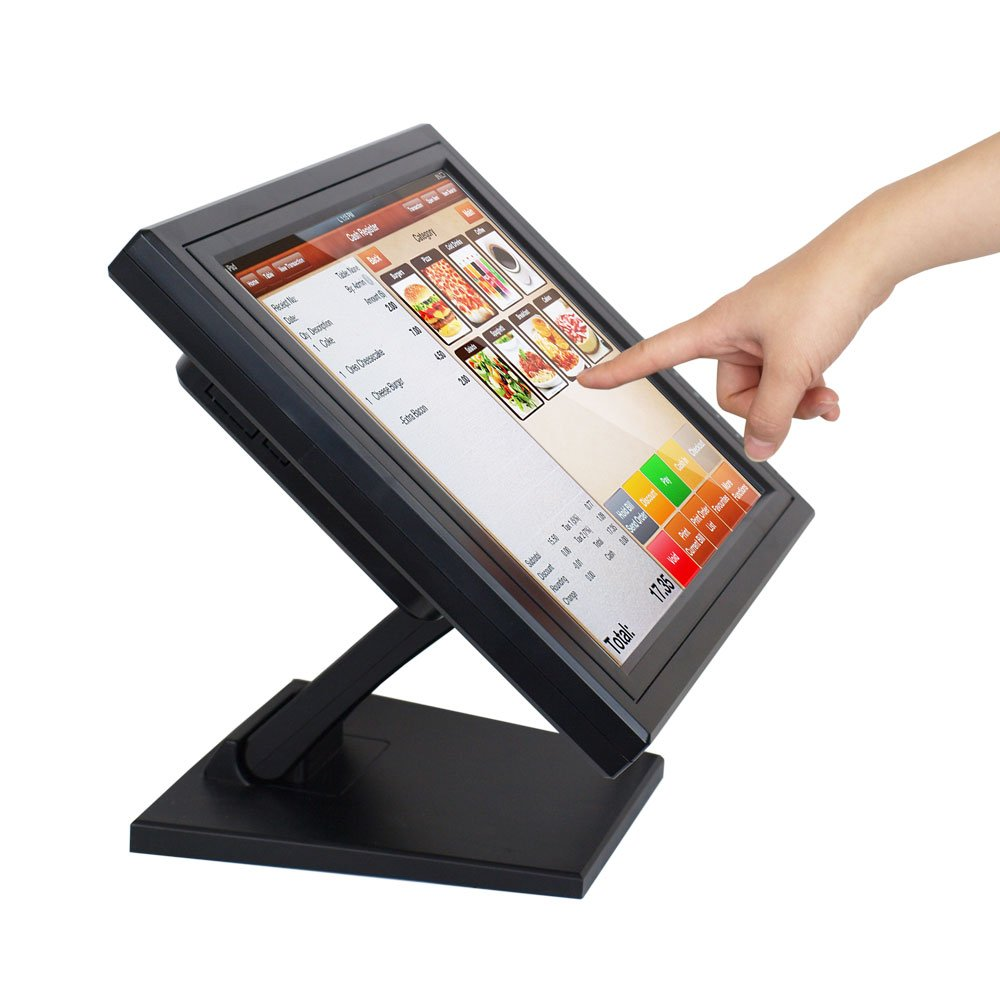
\includegraphics[width=\columnwidth]{img/touchscreen.jpg}
    \end{figure}
    Touchscreen
    \end{center}
\end{column}
\begin{column}{.22\textwidth}
  \begin{center} 
    \begin{figure}
      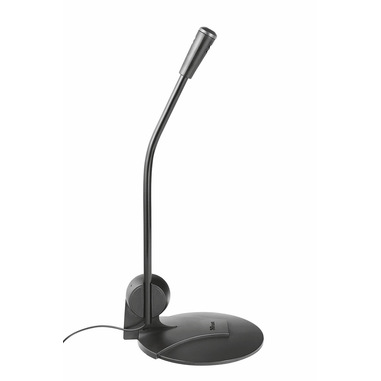
\includegraphics[width=\columnwidth]{img/microfono.jpg}
    \end{figure}
    Microfono
    \end{center}
\end{column}
\end{columns}
\end{frame}


\begin{frame}
\frametitle{Periferiche di output}
Queste periferiche permettono alla macchina di \alert<1>{restituire all'utente i risultati dell'elaborazione}.

~

\begin{columns}
\begin{column}{.22\textwidth}
  \begin{center}
  \begin{figure}
    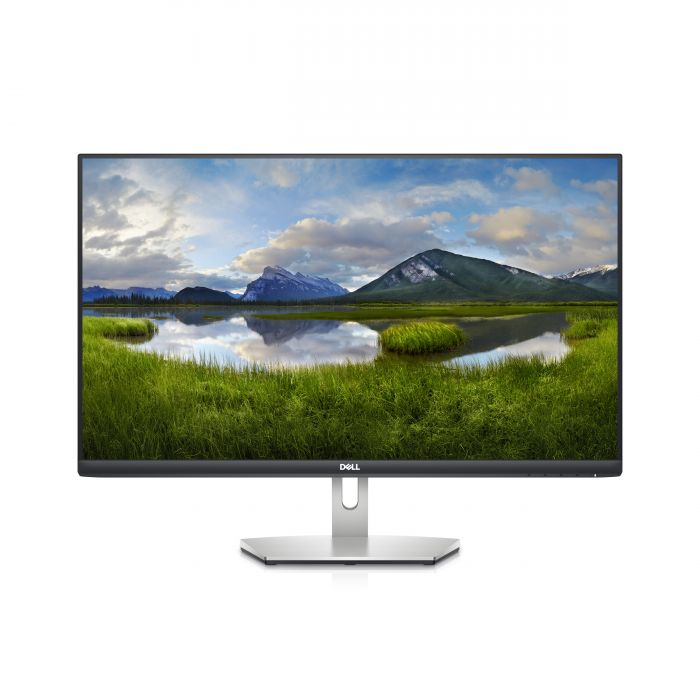
\includegraphics[width=\columnwidth]{img/monitor.jpg}
  \end{figure}
  Monitor
  \end{center}
\end{column}
\begin{column}{.22\textwidth}
  \begin{center}
    \begin{figure}
      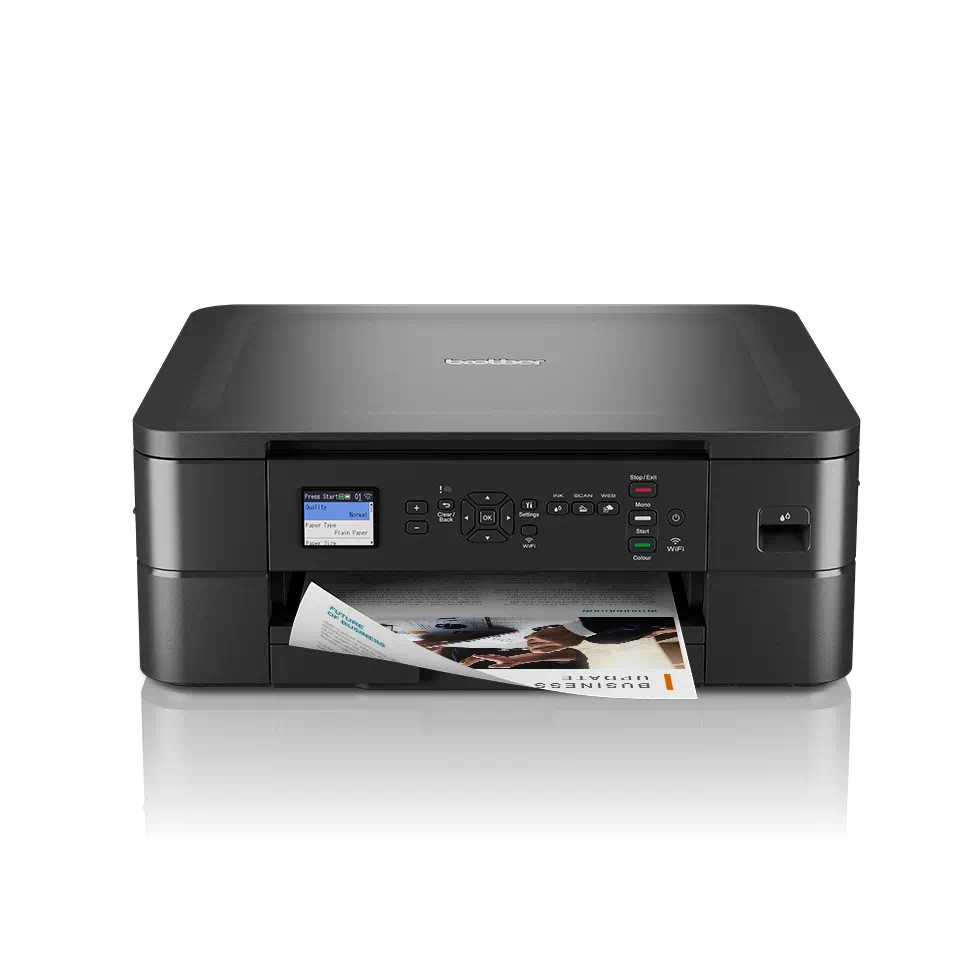
\includegraphics[width=\columnwidth]{img/stampante.jpg}
    \end{figure}
    Stampante
    \end{center}
\end{column}
\begin{column}{.22\textwidth}
  \begin{center} 
    \begin{figure}
      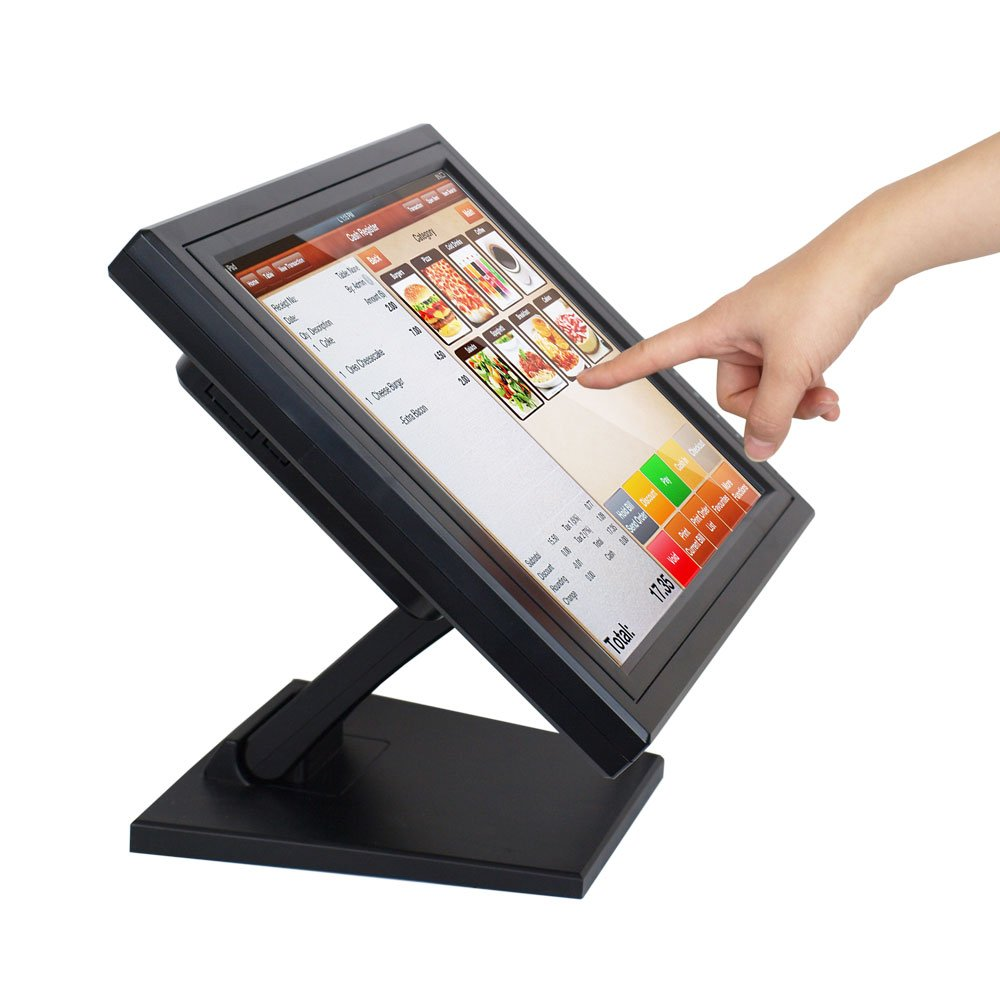
\includegraphics[width=\columnwidth]{img/touchscreen.jpg}
    \end{figure}
    Touchscreen
    \end{center}
\end{column}
\begin{column}{.22\textwidth}
  \begin{center} 
    \begin{figure}
      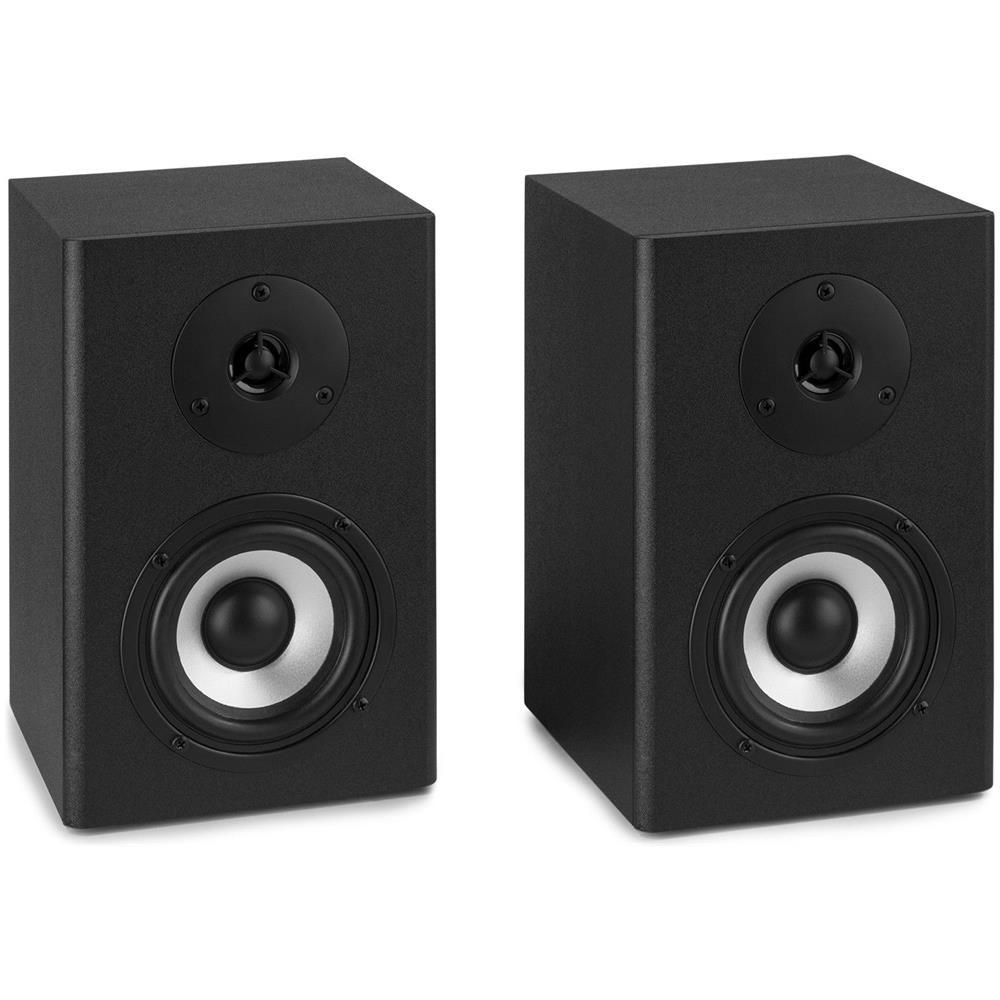
\includegraphics[width=\columnwidth]{img/casse.jpg}
    \end{figure}
    Casse
    \end{center}
\end{column}
\end{columns}
\end{frame}

\section{OS}

\begin{frame}
\frametitle{Il sistema operativo}
\begin{columns}
  \begin{column}{.65\textwidth}
    Il sistema operativo (OS, \emph{Operating System}) è l'\alert<1>{insieme dei programmi che gestiscono sia il software sia l'hardware del computer}.\pause

    ~
    
    Esempi di sistemi operativi sono Windows 10, MacOS, Ubuntu Linux, Android.\pause
    
    ~
    
    I sistemi operativi sono stati sviluppati (e continuano ad esserlo) per permettere agli utenti di \alert<3>{interagire agevolmente con la macchina}.
  \end{column}
  \begin{column}{.3\textwidth}
      \begin{figure}
        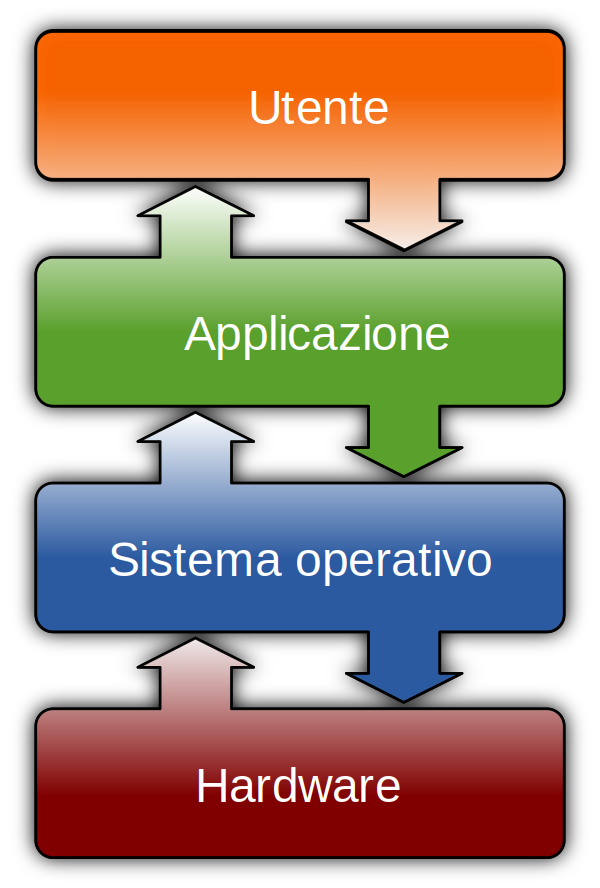
\includegraphics[width=\columnwidth]{img/sistemaoperativo.png}
      \end{figure}
  \end{column}
\end{columns}
\end{frame}


\begin{frame}
\frametitle{Windows}
Il SO Windows è stato sviluppato a partire dal 1985 dalla società Microsoft, di proprietà di Bill Gates.\pause

~

È un sistema \emph{closed source}, formato cioè da \alert<2>{software proprietario} che viene concesso in licenza all'utente.\pause

~

È presente sulla maggior parte dei computer per uso domestico, anche se risulta poco adatto ad applicazioni che richiedono una maggior sicurezza (ad es.~i server).

\begin{figure}
  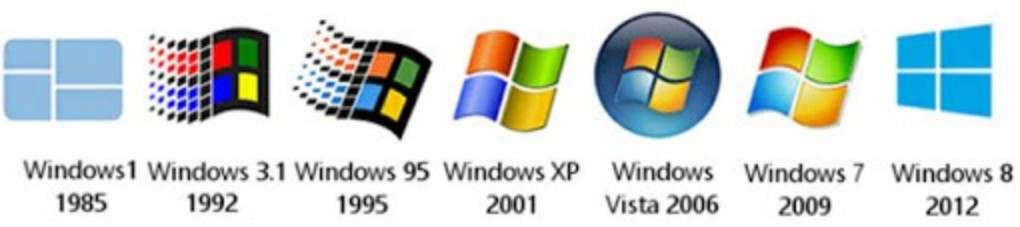
\includegraphics[width=.8\columnwidth]{img/windows.jpg}
\end{figure}
\end{frame}



\begin{frame}
\frametitle{Linux}
\begin{columns}
\begin{column}{.75\textwidth}
  Sviluppato da Linus Torvalds a partire dal 1991, ha un approccio al software molto diverso da quello di Windows.
\end{column}
\begin{column}{.15\textwidth}
  \begin{figure}
    
\includegraphics[width=\columnwidth]{img/tux.png}
  \end{figure}\pause
\end{column}
\end{columns}

~

Utilizza quasi esclusivamente software \alert<2>{open source}, cioè software il cui codice sorgente è liberamente disponibile per tutti gli utenti. Consente livelli di sicurezza molto maggiori di Windows.\pause

~

È completamente gratuito ed esiste in diverse versioni (dette ``distribuzioni''), a seconda delle necessità degli utenti.\pause

~

La versione più utilizzata su desktop è \alert<4>{Ubuntu Linux}, quella più utilizzata su server è \alert<4>{Debian}.
\end{frame}



\section{Formati}

\begin{frame}
\frametitle{Oggetti digitali}
Tutti gli oggetti digitali (acquisiti o creati con apparecchi digitali) vengono memorizzati su supporti di memoria.\pause

~

Sono dei \alert{files} identificati con:
\begin{itemize}
  \item un nome;\pause
  \item un'estensione, che ne specifica il formato.\pause
\end{itemize}

~

Esempio:
\begin{center}
  $ \underbrace{Chimica\_organica}.\underbrace{pdf} $\\
  ~~~~~~~~~ Nome del file ~~~ Estensione
\end{center}
\end{frame}




\begin{frame}
\frametitle{File di testo}
I formati più comuni per i file di testo sono:
\begin{itemize}
  \item TXT, per testo semplice;\pause
  \item DOC e DOCX, per testo formattato con Microsoft Word;\pause
  \item ODT, per testo formattato con LibreOffice o OpenOffice;\pause
  \item RTF, per testo formattato su diverse applicazioni;\pause
  \item PDF, per documenti che conservano il layout degli oggetti;\pause
  \item EPUB, per ebooks.
\end{itemize}
\end{frame}


\begin{frame}
\frametitle{File di immagini}
Le immagini possono essere in formato \alert<1>{bitmap} o \alert<1>{vettoriale}.\pause

~

I formati più comuni per le immagini sono:
\begin{itemize}
  \item BMP, per immagini create con MS Paint;\pause
  \item JPG e JPEG, per immagini compresse;\pause
  \item GIF, per sequenze di immagini compresse;\pause
  \item PNG, per immagini molto compresse;\pause
  \item PSD, per immagini modificabili in Photoshop;\pause
  \item SVG, per immagini vettoriali.
\end{itemize}
\end{frame}


\begin{frame}
\frametitle{File audio}
I suoni vengono digitalizzati con una certa \alert<1>{frequenza di campionamento} $ [Hz] $ e con una certa \alert<1>{profondità (risoluzione) di bit} [bps].\pause

~

I formati più comuni per l'audio sono:
\begin{itemize}
  \item WAV (lossless), usato per registrare professionalmente;\pause
  \item FLAC (lossless), per distribuire file audio di alta qualità;\pause
  \item WMA (lossy), formato Microsoft;\pause
  \item MP3 (lossy), formato compresso, buono oltre i 128 kb/s;\pause
  \item MIDI, per sequenze di suoni codificati.
\end{itemize}
\end{frame}


\begin{frame}
\frametitle{File video}
I filmati vengono digitalizzati con un certo \alert<1>{aspect ratio} (4:3, 16:9, \ldots) e con un certo numero di \alert<1>{fotogrammi per secondo} [fps].\pause

~

I formati più comuni per il video sono:
\begin{itemize}
  \item MPG e MPEG per video compressi;\pause
  \item MP4, evoluzione del precedente;\pause
  \item MOV, formato Apple;\pause
  \item AVI, formato compresso;\pause
  \item MKV, per video di alta qualità.
\end{itemize}
\end{frame}


\begin{frame}
\frametitle{Altri formati}
Altri formati notevoli sono:
\begin{itemize}
  \item XLS e ODS, per fogli di calcolo;\pause
  \item HTML, per pagine web;\pause
  \item CSS, per fogli di stile per pagine web;\pause
  \item ZIP, RAR e 7Z, per archivi compressi;\pause
  \item APK, per app Android.
\end{itemize}
\end{frame}




\end{document}
